\chapter{Introducción} \label{intro_chapter}

En este capítulo se hace un breve recorrido por la situación actual de la energía eólica en el país. Además, se introducen los conceptos básicos y principios de funcionamiento de la energía eólica y de los aerogeneradores. Se presentan el problema del control de una turbina eólica y la motivación en el diseño de un controlador que permita agregar un grado de libertad al sistema de la turbina. 
\\

\noindent En esta tesis se utilizarán indistintamente los términos aerogenerador y turbina eólica para referirse al conjunto completo del generador eléctrico, las aspas, el cuerpo de la turbina y demás componentes que se detallarán más adelante. 


\section{Contexto}
\noindent En la última década en México se ha visto un incremento en el consumo de energía primaria proveniente de fuentes renovables. Del 2012 al 2022 se registró un incremento de 5.24\% a 8.96\% la proporción del consumo de energía primaria cuyo origen se puede considerar renovable (i.e. energía solar, hidráulica, eólica, geotérmica, bioenergía y energía oceánica). Este incremento es en realidad una recuperación de las energías renovables a proporciones que habían sido observadas con anterioridad. En 1970 cerca del 11\% de la energía primaria consumida en el país provenía de fuentes renovables y desde entonces este indicador se ha mantenido oscilando entre 4-11\% \cite{statistical-review}.
\\

\noindent De forma similar, la producción de energía eléctrica en México proveniente de fuentes renovables a partir de 1985 y hasta 2022 ha fluctuado entre 15-32\% \cite{statistical-review}. En 2022 se registró una participación del 22.94\% de energías renovables en la generación de electricidad \cite{owid-renewable-energy}.
\\

\noindent A nivel mundial, la mayor parte de la generación de electricidad por medio de fuentes renovables se logra por medio de energía hidráulica - 4334.19 TWh (Terawatts hora) en 2022 -, y en segundo lugar se encuentra la energía eólica con 2104.84 TWh \cite{owid-renewable-energy}.
\\

\noindent En México se replica este patrón con 35.72 TWh generados por energía hidráulica y 20.32 TWh a partir de la energía del viento en este mismo año (2022) \cite{owid-renewable-energy}. Así mismo, la participación de la energía eólica en la generación de electricidad en el país pasó de 1.29\% en 2012 a 5.79\% en 2022. Desde el 2010 la generación de electricidad a través de energía eólica ha mostrado un crecimiento promedio de casi 35.49\% anual y este mismo periodo de tiempo solo ha mostrado una reducción en la generación entre el 2021 y el 2022 \cite{statistical-review}.
\\

\noindent De forma similar, la capacidad instalada de las centrales eólicas, definida como “la potencia que tiene una central eléctrica para generar electricidad considerando la disponibilidad técnica de sus instalaciones y de los insumos energéticos que serán transformados en electricidad en dichas instalaciones \cite{CONACYT2022}”, se ha incrementado a una tasa promedio de 28.72\% anual entre el 2010 y el 2022 \cite{statistical-review}.

\section{Breve introducción a las turbinas eólicas}

{\parindent0pt El uso del viento como fuente de energía no es reciente. Al contrario, su uso era conocido en varias de las civilizaciones anteriores a la era cristiana. Durante la edad media y hasta el siglo XVIII fueron populares los molinos de viento en varios países de Europa, principalmente los Países Bajos y Alemania. Este tipo de molinos también son los antecesores directos de las turbinas eólicas de eje horizontal que vemos hoy en día y que se encuentran en prácticamente todas las centrales de producción eléctrica en gran escala alrededor del mundo \cite{Hau2013}.
\\

El uso del viento en la generación de electricidad parece haber iniciado en Estados Unidos con la creación del primer aerogenerador de 12 kW por parte de Charles Bush \cite{Burton2011}, aunque también se consideran a otros inventores, como el danés Poul la Cour, como algunos de los pioneros en utilizar la energía del viento para generar electricidad \cite{Hansen2015}.
\\

Las turbinas eólicas modernas conservan el principio de funcionamiento de los primeros molinos de viento. Esto es, aprovechar la fuerza del viento para generar empuje en las aspas y producir un movimiento rotacional con el cual se pueda generar electricidad. Una mayor velocidad rotacional es deseable dado que reduce la relación de la caja de cambios del rotor. Sin embargo, como se verá más adelante, una velocidad rotacional demasiado alta puede generar demasiado estrés en el generador u otros componentes y conducir a fallos por parte del aerogenerador. 
\\

En 2009 la Asociación Europea de Energía Eólica (EWEA) realizó el balance de energía asociado a un aerogenerador de 3 MW concluyendo que el tiempo promedio en el que dicho aerogenerador produciría la energía equivalente a su producción, operación, transporte y desmantelamiento es de 6 a 7 meses \cite{Burton2011}.
\\

Para la producción de energía a gran escala son más comunes los aerogeneradores de eje horizontal que aquellos de eje vertical (véase figura \ref{VAWT}). Lo anterior debido a distintos factores que favorecen la configuración horizontal del generador entre los que destacan:

\begin{itemize}
\item La posibilidad de controlar la velocidad y potencia otorgadas por el generador a partir de modificar el ángulo de ataque de las aspas del generador, lo cual resulta ser la forma más eficiente de limitar la velocidad angular particularmente en turbinas de gran tamaño.
\item La forma de las aspas se puede diseñar para que sea aerodinámica y, de esta forma, aprovechar mejor toda la energía del viento
\item La existencia de más y mejor tecnología para turbinas de eje horizontal \cite{Hau2013}.
\end{itemize}

\begin{figure}[H]
    \centering
    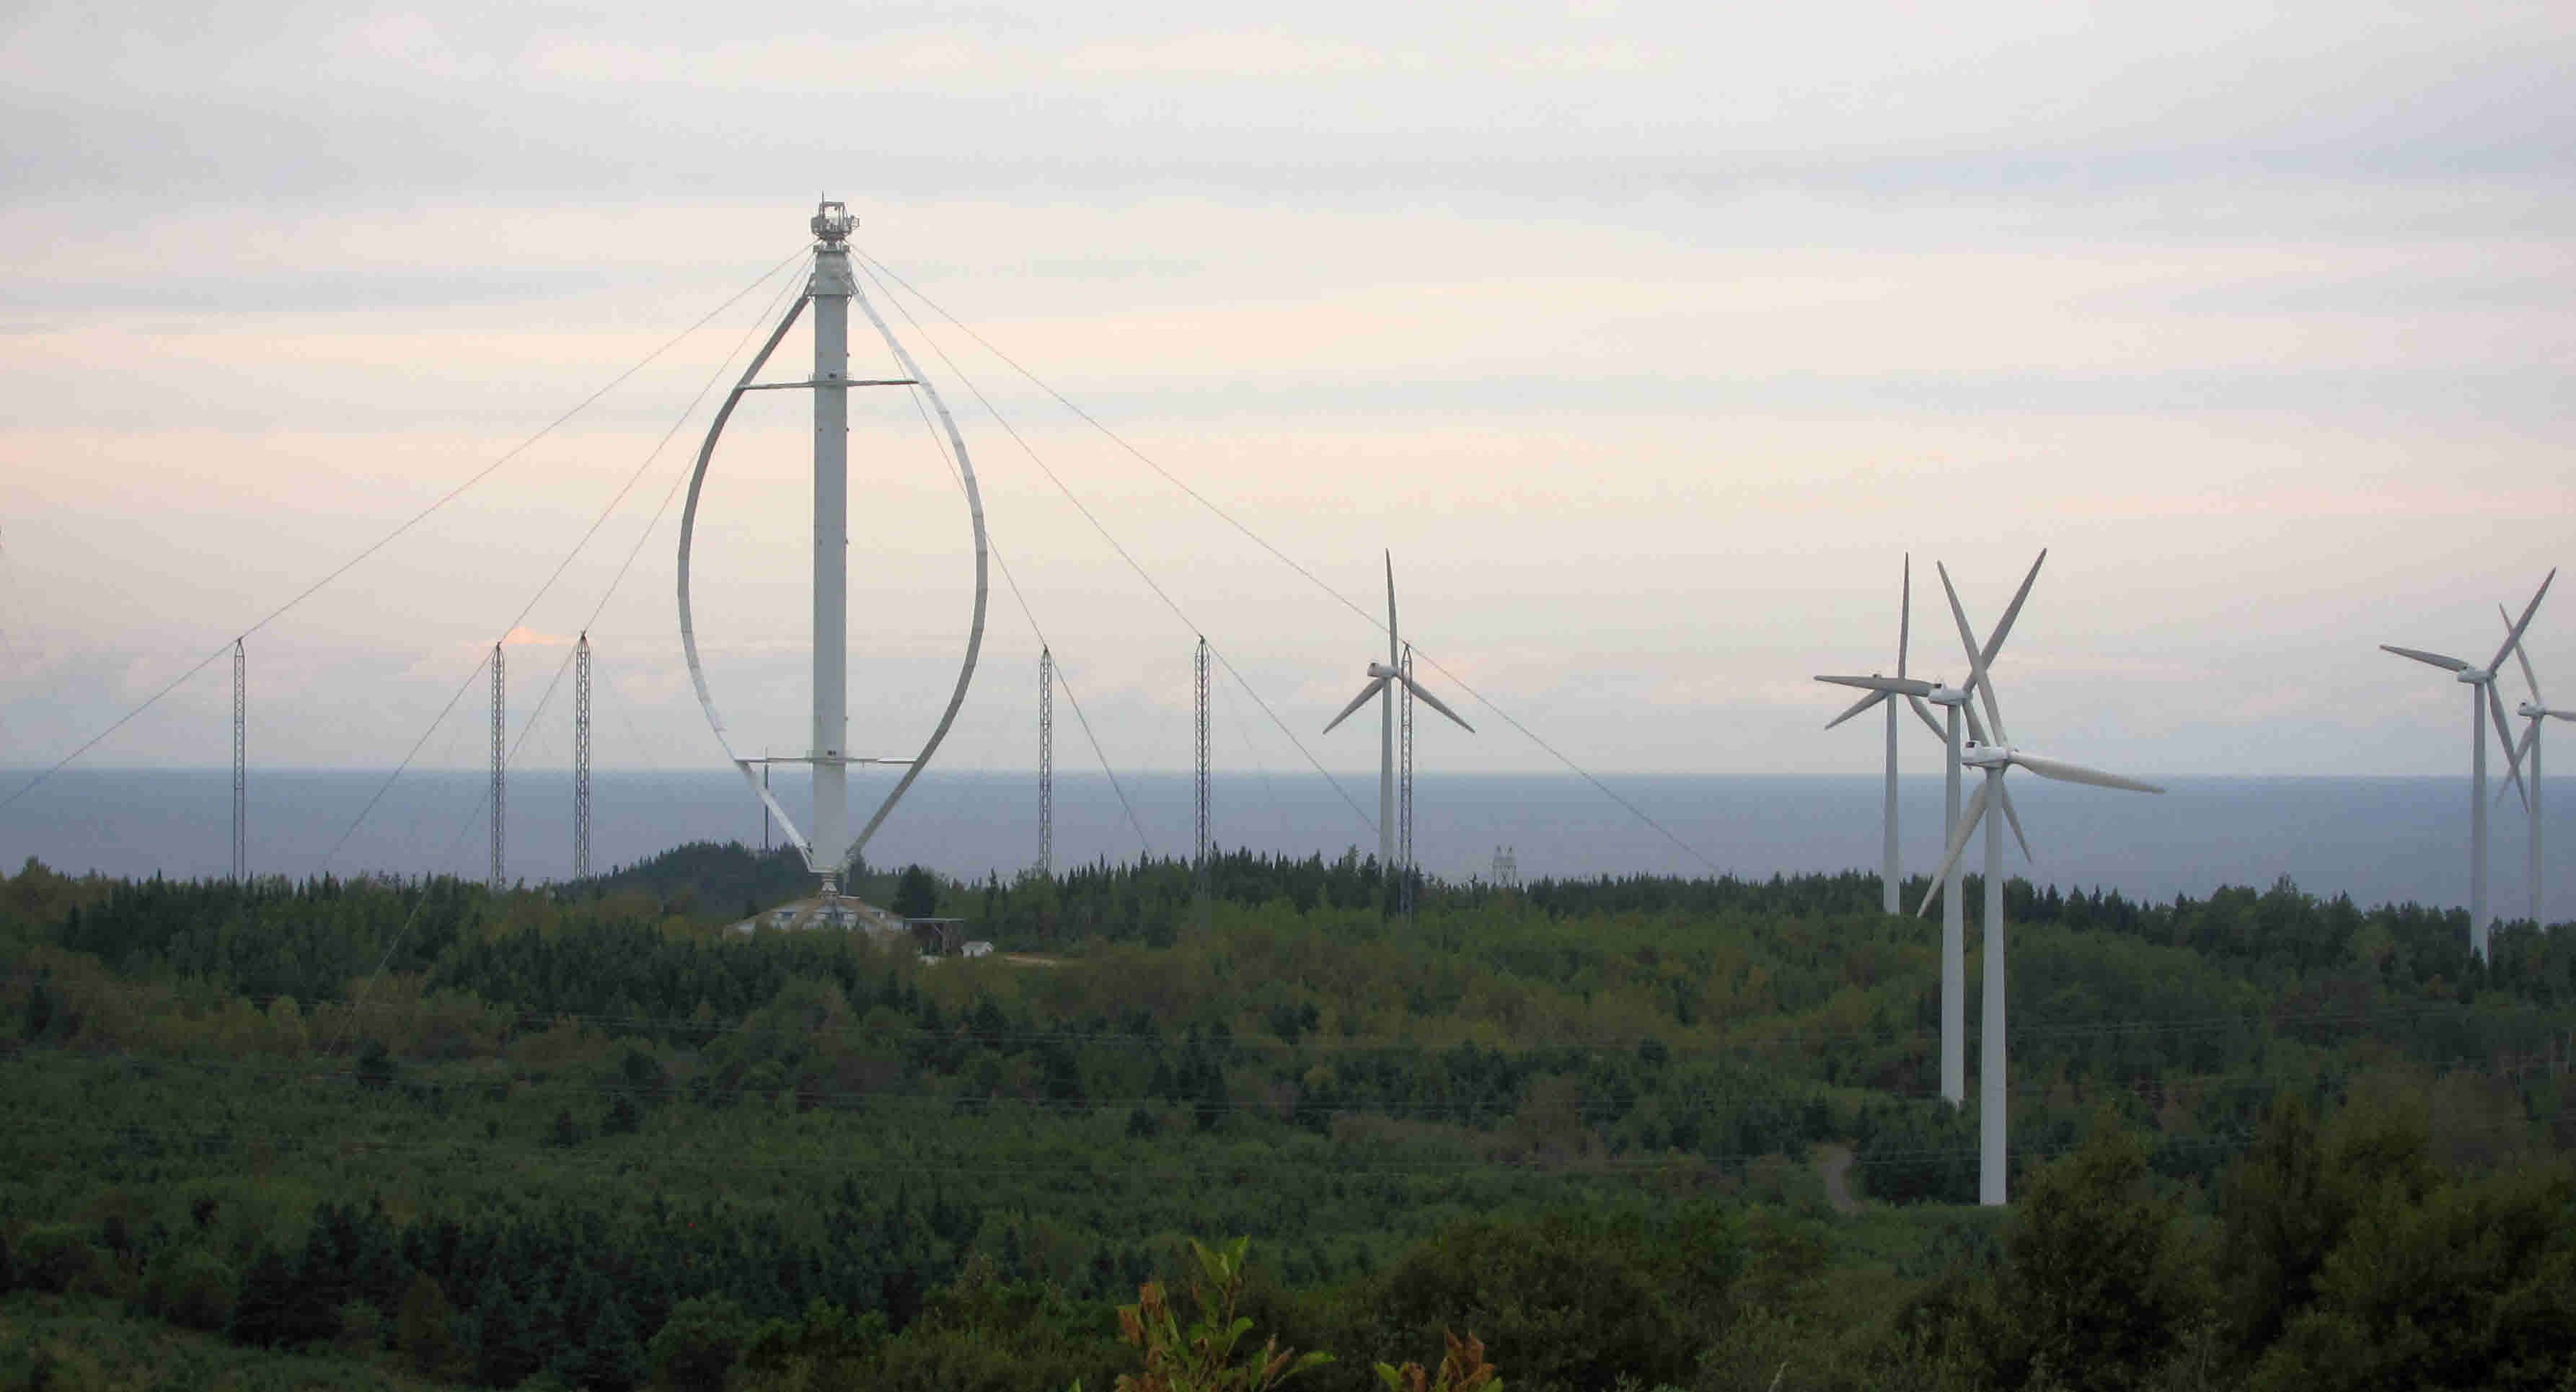
\includegraphics[width=0.9\textwidth]{Imagenes/Eole_cap-chat.jpeg}
    \caption{\small{\textbf{Aerogeneradores de eje vertical y horizontal:} Pierre5018, CC BY-SA 4.0 (https://creativecommons.org/licenses/by-sa/4.0), vía Wikimedia Commons}}
    \label{VAWT}
\end{figure}

Los aerogeneradores de eje horizontal tienen 3 componentes principales: la torre, el rotor y la góndola (\emph{nacelle}). Dentro de la góndola se encuentra el generador eléctrico conectado con el rotor por medio de los ejes de alta y baja velocidad, así como la caja de cambios (\emph{gearbox}) \cite{Pao2009}. La mayoría de las turbinas eólicas de gran escala cuentan con un sistema que permite girar la góndola y el rotor para que apunte siempre en la dirección del viento, este sistema es manejado por el \emph{yaw actuator} y une la góndola con la torre. El rotor incluye las aspas y, en algunos casos, los actuadores que controlan el ángulo de estas (\emph{pitch actuator}). 
\\

Las turbinas eólicas pueden ser de velocidad fija o variable. Las turbinas de velocidad variable puede trabajar más cerca de la máxima eficiencia aerodinámica por un mayor tiempo. Sin embargo, el hecho de tener una velocidad variable implica también que se debe realizar una correcta regulación y procesamiento de la electricidad generada para que esta pueda ser subida a la red con la frecuencia correcta \cite{Pao2009}.
\\

Las turbinas de velocidad variable suelen trabajar en 3 regiones de operación. Cuando la velocidad del viento es baja (usualmente menor a 6 $\text{m}/\text{s}$) la potencia del viento es insuficiente y las turbinas suelen permanecer detenidas. A esto se le conoce como \textbf{región 1} e incluye también el momento en el que las turbinas se encienden y comienzan a girar. Durante la región 1 el control se limita al monitoreo y supervisión de la velocidad del viento para determinar en qué momento se pueden iniciar las rutinas de activación para encender las turbinas \cite{Johnson2004}.
\\

La \textbf{región 2} de operación ocurre generalmente cuando el viento alcanza velocidades entre 5 y 14 $\text{m}/\text{s}$. En esta región se busca extraer la mayor potencia posible del viento y para esto se pueden utilizar cualquiera de los tipos de control disponibles en el aerogenerador (\emph{yaw control}, \emph{pitch control} y \emph{torque control}). Debido a que las velocidades del viento son menores que las presentadas en la región 3 normalmente no es necesario reducir las cargas [mecánicas y eléctricas] cuando la turbina opera en la región 2 \cite{Johnson2004}.
\\

Por último, la \textbf{región 3} ocurre cuando el viento supera la velocidad a la cual se extrae la potencia máxima por el aerogenerador. Aunque la velocidad del viento siga aumentando, las turbinas deben limitar la potencia que se extrae del viento para evitar daños en sus componentes debido al estrés y las cargas producidas por la fuerza del viento \cite{Pao2009}-\cite{Johnson2004}. De aquí que la gráfica potencia-velocidad se vea plana en la región 3 (ver figura \ref{Regiones}) aun cuando el viento se siga incrementando hasta alcanzar un cierto valor límite (\emph{high wind cutout}). Después de este límite las turbinas deben ser detenidas completamente.
\\
\begin{figure}[H]
    \centering
    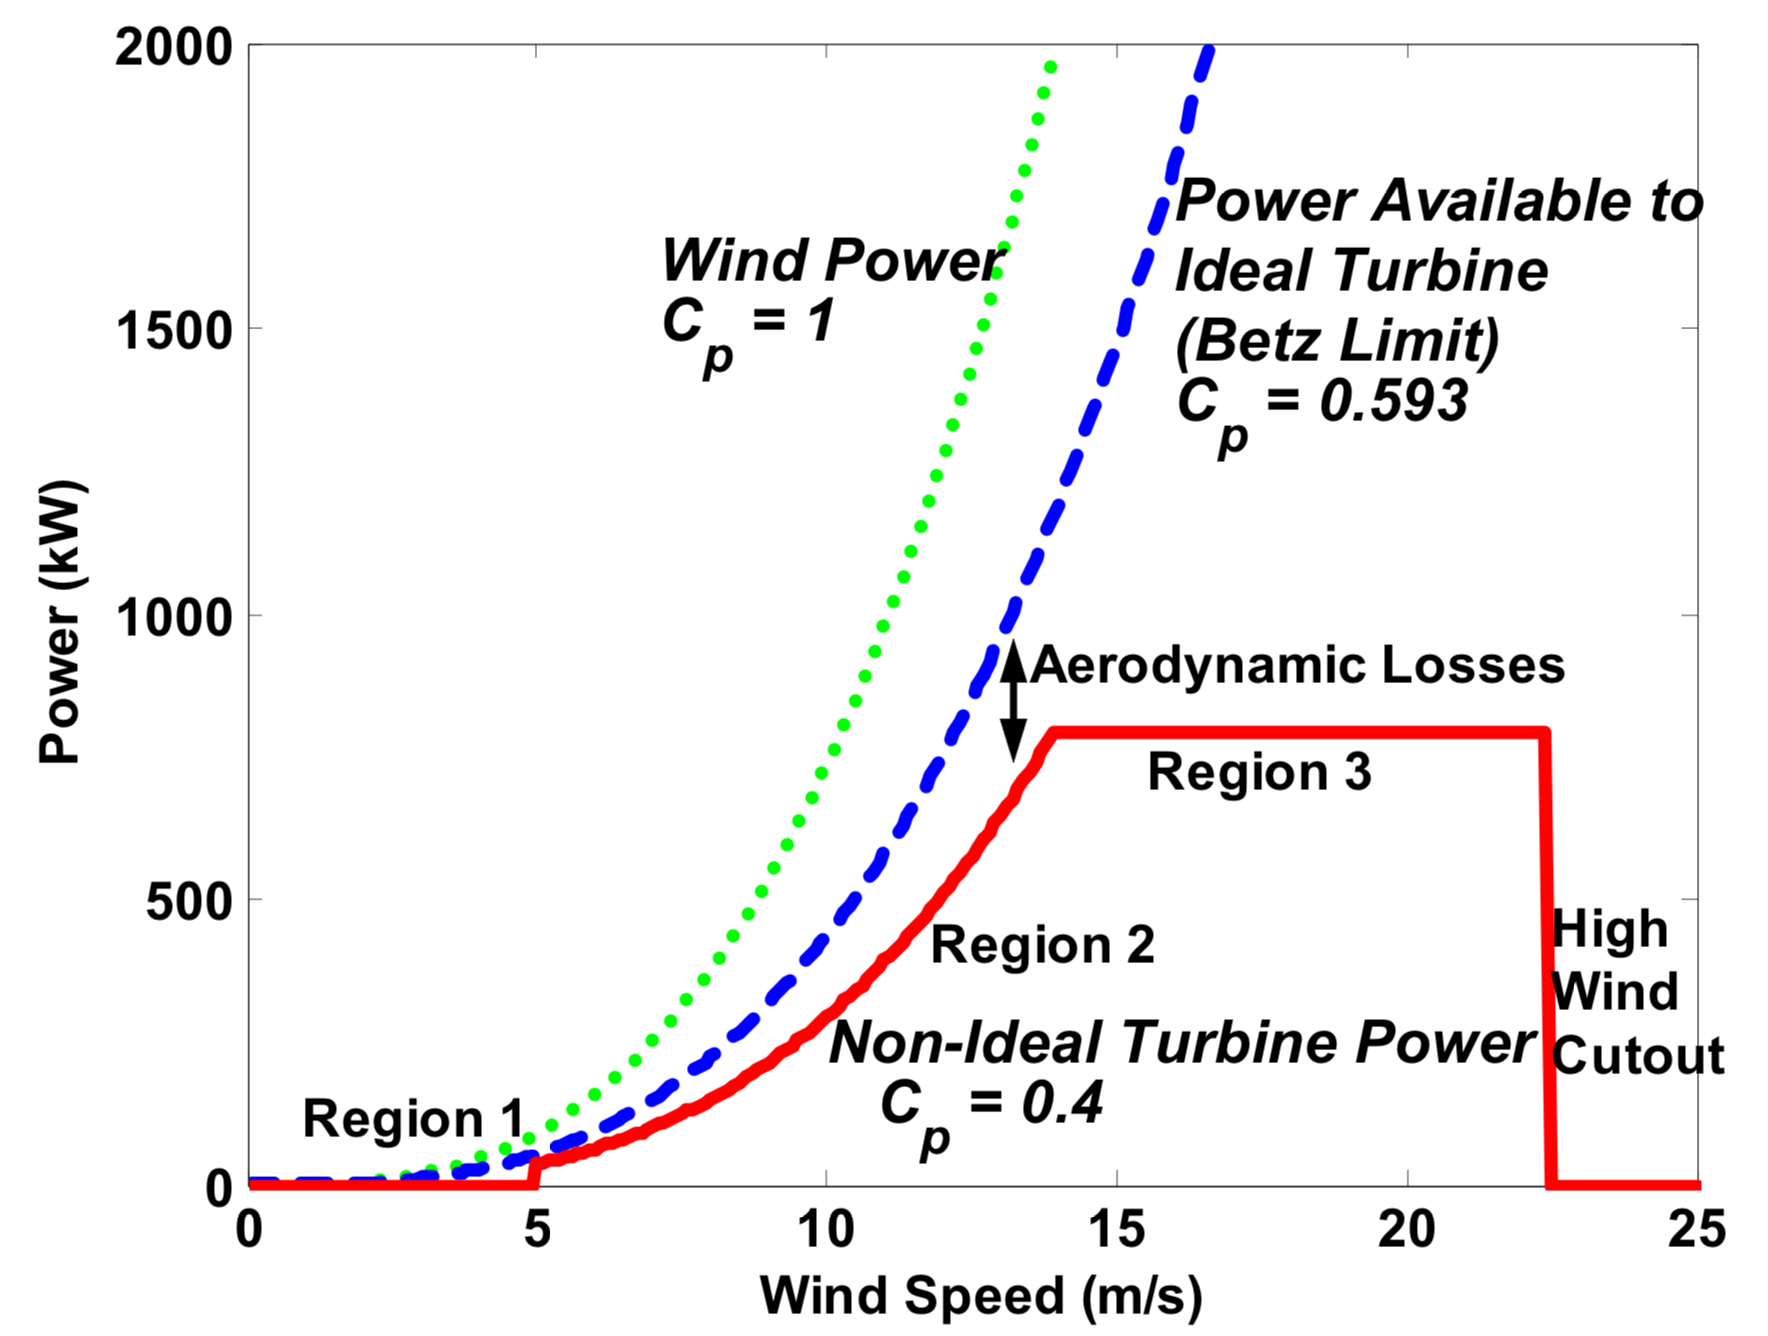
\includegraphics[width=0.8\textwidth]{Imagenes/Regions.jpeg}
    \caption{Regiones de control de un aerogenerador \cite{Johnson2004}}
    \label{Regiones}
\end{figure}

Adicionalmente, las turbinas eólicas tienen una eficiencia definida como el porcentaje de la potencia del viento que de hecho puede ser aprovechada por la turbina eólica. La eficiencia máxima alcanzable de manera teórica está dada por el número de Betz $B=\frac{16}{27}\approx 59.26$\% \cite{Huleihil2012}. Esto implica que solo el 59\% de la potencia del viento puede ser realmente convertida en energía eléctrica. Este valor es teórico y en la práctica las turbinas eólicas suelen tener valores de eficiencia entre 35-45\%.
}

\section{Identificación del problema}
{\parindent0pt
El problema del control de una turbina eólica puede ser tratado desde distintos ángulos. Aquella magnitud física que se maneje como variable de control definirá el alcance y el tipo del control que se vaya a realizar. 
\\

Las turbinas eólicas producidas en los últimos años incluyen actuadores para cada una de las aspas, lo que provee una nueva forma de controlar la generación de energía además de la forma tradicional que implica el control del par eléctrico del generador \cite{Laks2009}.
\\

Durante el ciclo de operación de un aerogenerador, este debe poder adaptarse a los cambios constantes e impredecibles del viento, tanto en su dirección como en su velocidad. Para esto se han implementado sistemas de control que van desde el \emph{yaw control} que permite que el conjunto completo de la góndola y el rotor giren sobre la torre para que mantener el viento normal al plano del rotor; hasta el \emph{pitch control} que permite girar las aspas para modificar el ángulo con el que el viento choca contra la superficie aerodinámica de cada aspa. 
\\

Otra forma de enfrentar el problema de la velocidad del viento —y, por tanto, del torque recibido por el rotor— es a través de controlar el par eléctrico del generador (\emph{torque control}), lo que permite controlar la cantidad de torque que se demanda del rotor y de esta forma optimizar su velocidad \cite{Johnson2004}.
\\

Cuando el viento muestra velocidades por debajo del límite establecido para ciertos aerogeneradores en específico, estos suelen realizar el control de velocidad del rotor por medio del \emph{yaw control} y el control del par eléctrico, manteniendo el ángulo de ataque de las aspas a un valor fijo calculado como el óptimo en el cual se extrae la mayor cantidad de energía del viento. Sin embargo, cuando el viento alcanza velocidades más altas que el valor límite se vuelve importante reducir las cargas mecánicas y eléctricas para no superar sus valores máximos considerados en el diseño de dichos componentes. 
\\

La principal consecuencia de alcanzar las velocidades límites del viento es que usualmente conlleva a que los aerogeneradores sean frenados hasta quedar completamente detenidos. Lo anterior para evitar daños a sus componentes debido a las cargas excesivas, considerando además que las turbinas eólicas modernas tienen costos bastante altos asociados tanto a su producción como a su mantenimiento. Esto puede resultar contraproducente dado que los aerogeneradores permanecen detenidos en aquellos momentos en que la generación de energía eléctrica es teóricamente mayor y, por tanto, se está desperdiciando toda esa potencia del viento.


}


\section{Objetivo}
\noindent De lo anterior, la presente tesis tiene como objetivos los siguientes puntos:
\begin{enumerate}
\item Encontrar una ley de control que, manipulando el ángulo de ataque de las aspas, permita regular el par mecánico.
\item Considerar el escenario en el que se requiere extraer la máxima potencia proveniente del viento, procedimiento conocido como MPTT (Maximum Power Point Tracking). Este punto requiere que el aerogenerador rote a cierta velocidad que en la práctica se desconoce.
\item Agregar al modelo la parte eléctrica y encontrar una ley de control que permita regular el par eléctrico al manipular la carga. Luego, hacer operar de manera conjunta ambas partes, la eléctrica y la mecánica, con sus respectivas leyes de control. 
\end{enumerate}


\section{Metodología}

\noindent Para el desarrollo de esta tesis se seguirán la metodología ágil. En particular la variante de la metodología ágil conocida como SCRUM. La elección debido a que su organización en \emph{sprints} cortos con versiones listas para entregar permite enfocar la atención en un problema a la vez y trabajar sobre este hasta resolverlo. De esta forma el esfuerzo se concentra en una etapa del proyecto y hasta que esta esté concluida se avanza con las posteriores. La metodología ágil SCRUM facilita también el desarrollo de proyectos de alta complejidad y en los que se incursiona en áreas poco conocidas para los colaboradores. 